\documentclass{beamer}
\usepackage[utf8]{inputenc}
\usepackage[T1]{fontenc}
\usepackage[norsk]{babel}
\usepackage{hyperref}
\usepackage{fancyvrb}


\usepackage{tikz}
\usepackage{amsmath}

\usetikzlibrary{shapes}
\usetikzlibrary{automata}
\usetikzlibrary{calendar}
\usetikzlibrary{mindmap}

\begin{document}

\begin{frame}
\begin{center}
\Huge{Tegnekurs i Ti\textit{k}Z} \\
\vspace{10pt}
\Large{Veronika Heimsbakk}\\
veronika.heimsbakk@acando.no
\end{center}
\end{frame}

\begin{frame}{Om meg}
\begin{itemize}
\item
Systemutvikler i Acando innen semantiske teknologier.
\item
Ferdig på Ifi V2015.
\item
Forkjærlighet for Ti\textit{k}Z, \LaTeX{} og typografi.
\end{itemize}
\end{frame}

%%% THE BASICS : LAGE TIKZPICTURE%%%
\begin{frame}[fragile]
\frametitle{The Basics}

Inkludere pakken:
\begin{Verbatim}[fontsize=\small]
\usepackage{tikz}
\end{Verbatim}

\vspace{20pt}

Opprette miljøet:
\begin{Verbatim}[fontsize=\small]
\begin{tikzpicture}
    <kode her>
\end{tikzpicture}
\end{Verbatim}

\end{frame}

%%% THE BASICS : LINJE%%%
\begin{frame}[fragile]
\frametitle{The Basics -- tegne ei linje}
\begin{center}
\begin{tikzpicture}
	\draw (0,0) -- (4,0);
\end{tikzpicture}
\end{center}

\begin{itemize}
\item
\begin{Verbatim}[fontsize=\small]
\draw (0,0) -- (4,0);
\end{Verbatim}
\end{itemize}

\begin{center}
\begin{tikzpicture}
	\draw (0em,0em) -- (4em,0em);
\end{tikzpicture}
\end{center}

\begin{itemize}
\item
\begin{Verbatim}[fontsize=\small]
\draw (0em,0em) -- (4em,0em);
\end{Verbatim}
\end{itemize}

\begin{center}
\begin{tikzpicture}
	\draw (0pt,0pt) -- (4pt,0pt);
\end{tikzpicture}
\end{center}

\begin{itemize}
\item
\begin{Verbatim}[fontsize=\small]
\draw (0pt,0pt) -- (4pt,0pt);
\end{Verbatim}
\end{itemize}

\end{frame}

%%% THE BASICS : KURVER%%%
\begin{frame}[fragile]
\frametitle{The Basics -- kvadrat}
\begin{center}

\begin{tikzpicture}
	\draw[black, very thick] (-2,2) .. controls (-1,0) and (1,0) .. (2,2);
\end{tikzpicture}
\end{center}

\vspace{20pt}

\begin{Verbatim}[fontsize=\small]
\draw (-2,2) .. controls (-1,0) and (1,0) .. (2,2);
\end{Verbatim}

\end{frame}

%%% THE BASICS : KVADRAT%%%
\begin{frame}[fragile]
\frametitle{The Basics -- kvadrat}
\begin{center}
\begin{tikzpicture}
	\draw (0,0) rectangle (4,4);
\end{tikzpicture}
\end{center}

\vspace{20pt}
\begin{itemize}
\item
\begin{Verbatim}[fontsize=\small]
\draw (0,0) -- (4,0) -- (4,4) -- (0,4) -- (0,0);
\end{Verbatim}

\item
\begin{Verbatim}[fontsize=\small]
\draw (0,0) rectangle (4,4);
\end{Verbatim}
\end{itemize}
\end{frame}

%%% THE BASICS : SIRKEL%%%
\begin{frame}[fragile]
\frametitle{The Basics -- sirkel}
\begin{center}
\begin{tikzpicture}
	\draw (2,2) circle (1.5cm);
	\draw (6,2) ellipse (2cm and 1cm);
\end{tikzpicture}
\end{center}

\vspace{20pt}

\begin{itemize}
\item
\begin{Verbatim}[fontsize=\small]
\draw (0,0) circle (1.5cm);
\end{Verbatim}

\item
\begin{Verbatim}[fontsize=\small]
\draw (0,0) ellipse (2cm and 1cm);
\end{Verbatim}
\end{itemize}

\end{frame}

%%% THE BASICS : SIRKEL PYNT%%%
\begin{frame}[fragile]
\frametitle{The Basics -- pynte litt}
\begin{center}

\begin{tikzpicture}
	\draw[red, very thick, dashed] (2,2) circle (1.5cm);
	\draw[green, thick] (6,2) circle (1.5cm);
\end{tikzpicture}
\end{center}

\vspace{20pt}

\begin{itemize}
\item
\begin{Verbatim}[fontsize=\small]
\draw[red, very thick, dashed] (0,0) circle (1.5cm);
\end{Verbatim}

\item
\begin{Verbatim}[fontsize=\small]
\draw[green, thick] (0,0) circle (1.5cm);
\end{Verbatim}
\end{itemize}

\end{frame}

%%% THE BASICS : TYKKELSER%%%
\begin{frame}[fragile]
\frametitle{The Basics -- tykkelser}
\begin{center}
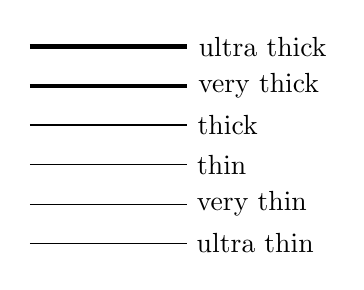
\begin{tikzpicture}
	\draw[ultra thin] (0,0) -- (2,0) node[right] {ultra thin};
	\draw[very thin] (0,0.5) -- (2,0.5) node[right] {very thin};
	\draw[thin] (0,1) -- (2,1) node[right] {thin};
	\draw[thick] (0,1.5) -- (2,1.5) node[right] {thick};
	\draw[very thick] (0,2) -- (2,2) node[right] {very thick};'
	\draw[ultra thick] (0,2.5) -- (2,2.5) node[right] {ultra thick};
\end{tikzpicture}
\end{center}

\end{frame}

%%% THE BASICS : FARGER%%%
\begin{frame}[fragile]
\frametitle{The Basics -- farger}
\begin{center}
\scalebox{0.8}{
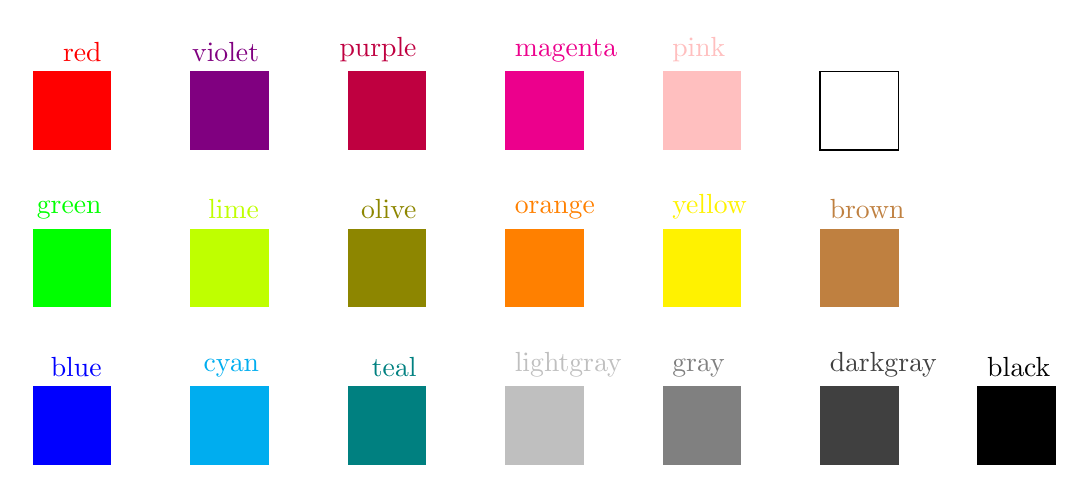
\begin{tikzpicture}
	\fill[red] (0,4) rectangle (1,5) node[above left] {red};
	\fill[violet] (2,4) rectangle (3,5) node[above left] {violet};
	\fill[purple] (4,4) rectangle (5,5) node[above left] {purple};
	\fill[magenta] (7,4) rectangle (6,5) node[above right] {magenta};
	\fill[pink] (9,4) rectangle (8,5) node[above right] {pink};
	\fill[white, draw=black, thin] (11,4) rectangle (10,5) node[above right] {white};

	\fill[green] (0,2) rectangle (1,3) node[above left] {green};
	\fill[lime] (2,2) rectangle (3,3) node[above left] {lime};
	\fill[olive] (4,2) rectangle (5,3) node[above left] {olive};
	\fill[orange] (7,2) rectangle (6,3) node[above right] {orange};
	\fill[yellow] (9,2) rectangle (8,3) node[above right] {yellow};
	\fill[brown] (11,2) rectangle (10,3) node[above right] {brown};

	\fill[blue] (0,0) rectangle (1,1) node[above left] {blue};
	\fill[cyan] (2,0) rectangle (3,1) node[above left] {cyan};
	\fill[teal] (4,0) rectangle (5,1) node[above left] {teal};
	\fill[lightgray] (7,0) rectangle (6,1) node[above right] {lightgray};
	\fill[gray] (9,0) rectangle (8,1) node[above right] {gray};
	\fill[darkgray] (11,0) rectangle (10,1) node[above right] {darkgray};
	\fill[black] (13,0) rectangle (12,1) node[above right] {black};
\end{tikzpicture}
}
\end{center}

\end{frame}

%%% THE BASICS : FARGER%%%
\begin{frame}[fragile]
\frametitle{The Basics -- fylle med farge}
\begin{center}
\begin{center}

\begin{tikzpicture}
	\fill[orange] (0,0) rectangle (2,2);
\end{tikzpicture}
\end{center}
\end{center}

\vspace{20pt}

\begin{Verbatim}[fontsize=\small]
\fill[orange] (0,0) rectangle (2,2);
\end{Verbatim}

\end{frame}

\begin{frame}[fragile]
\frametitle{The Basics -- fylle med farge og kant}
\begin{center}

\begin{tikzpicture}
	\filldraw[orange!50, draw=black, very thick] (0,0) rectangle (2,2);
\end{tikzpicture}
\end{center}


\vspace{20pt}

\begin{Verbatim}[fontsize=\footnotesize]
\filldraw[orange!50, draw=black, very thick] (0,0) rectangle (2,2);
\end{Verbatim}

\end{frame}

\begin{frame}[fragile]
\frametitle{The Basics -- fylle med gradient}
\begin{center}

\begin{tikzpicture}
	\shade[left color=orange, right color=yellow] (0,0) rectangle (2,2);
	\shade[top color=orange, bottom color=yellow] (3,0) rectangle (5,2);
	\shade[inner color=orange, outer color=yellow] (6,0) rectangle (8,2);
\end{tikzpicture}
\end{center}

\vspace{20pt}

\begin{Verbatim}[fontsize=\footnotesize]
\shade[left color=orange, right color=yellow] (0,0) rectangle (2,2);
\shade[top color=orange, bottom color=yellow] (3,0) rectangle (5,2);
\shade[inner color=orange, outer color=yellow] (6,0) rectangle (8,2);
\end{Verbatim}

\end{frame}

\begin{frame}[fragile]
\frametitle{The Basics -- blande farger}
\begin{center}
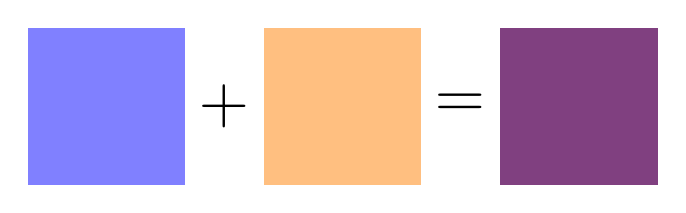
\begin{tikzpicture}
	\fill[blue!50] (0,0) rectangle (2,2);
	\node[black] (1) at (2.5,1) {\Huge{+}};
	\fill[orange!50] (3,0) rectangle (5,2);
	\node[black] (1) at (5.5,1) {\Huge{=}};
	\fill[blue!50!orange] (6,0) rectangle (8,2);
\end{tikzpicture}
\end{center}

\vspace{20pt}

\begin{Verbatim}[fontsize=\small]
\fill[blue!50!orange] (0,0) rectangle (0,0);
\end{Verbatim}

\end{frame}


%%% PILER %%%
\begin{frame}[fragile]
\frametitle{Piler i TikZ}
\begin{center}
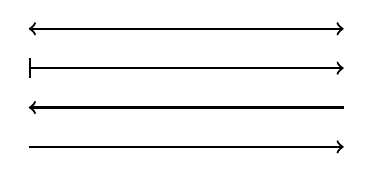
\begin{tikzpicture}
    \draw[->, thick] (0,0) -- (4,0);
    \draw[<-, thick] (0,0.5) -- (4,0.5);
    \draw[|->, thick] (0,1) -- (4,1);
    \draw[<->, thick] (0,1.5) -- (4,1.5);
\end{tikzpicture}
\end{center}

\vspace{20pt}

\begin{Verbatim}[fontsize=\small]
\draw[<->] (0,1.5) -- (4,1.5);
\draw[|->] (0,1) -- (4,1);
\draw[<-]  (0,0.5) -- (4,0.5);
\draw[->]  (0,0) -- (4,0);
\end{Verbatim}

\end{frame}

%%% PLOTTE FUNKSJONER %%%
\begin{frame}[fragile]
\frametitle{Plotte funksjoner}
\begin{center}
\begin{tikzpicture}
    \draw[<->] (0,3.5) -- (0,0) -- (5,0);
    \draw[red, thick, domain=0:1.2] plot (\x, {0.25+\x+\x*\x});
\end{tikzpicture}
\end{center}

\vspace{20pt}

\begin{Verbatim}[fontsize=\footnotesize]
\begin{tikzpicture}
    \draw[<->] (0,3.5) -- (0,0) -- (5,0);
    \draw[red, thick, domain=0:1.2] plot (\x, {0.25+\x+\x*\x});
\end{tikzpicture}
\end{Verbatim}

\end{frame}

%%% KOORDINATSYSTEM: RUTENETT%%%
\begin{frame}[fragile]
\frametitle{Rutenett med akser}
\begin{center}
\scalebox{0.5}{%
\begin{minipage}{\textwidth}
\begin{tikzpicture}
    \draw[step=1cm,gray,very thin] (-1.9,-1.9) grid (5.9,5.9);
\end{tikzpicture}
\end{minipage}%
}  
\end{center}

\vspace{20pt}

\begin{Verbatim}[fontsize=\small]
\draw[step=1cm,gray,very thin] (-1.9,-1.9) grid (5.9,5.9);
\end{Verbatim}

\end{frame}

%%% KOORDINATSYSTEM: AKSER%%%
\begin{frame}[fragile]
\frametitle{Rutenett med akser}
\begin{center}
\scalebox{0.5}{%
\begin{minipage}{\textwidth}
\begin{center}
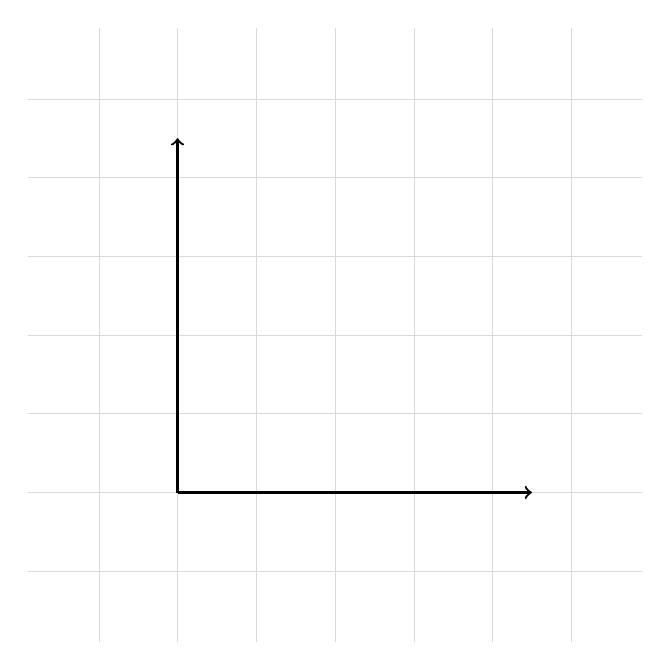
\begin{tikzpicture}
    \draw[step=1cm,gray!30,very thin] (-1.9,-1.9) grid (5.9,5.9);
    \draw[thick, ->] (0,0) -- (4.5,0);
    \draw[thick, ->] (0,0) -- (0,4.5);
\end{tikzpicture}
\end{center}
\end{minipage}%
}  
\end{center}

\vspace{20pt}

\begin{Verbatim}[fontsize=\small]
\draw[step=1cm,gray!30,very thin] (-1.9,-1.9) grid (5.9,5.9);
\draw[thick, ->] (0,0) -- (4.5,0);
\draw[thick, ->] (0,0) -- (0,4.5);
\end{Verbatim}

\end{frame}

%%% KOORDINATSYSTEM: LABEL%%%
\begin{frame}[fragile]
\frametitle{Rutenett med akser}
\begin{center}
\scalebox{0.5}{%
\begin{minipage}{\textwidth}
\begin{center}

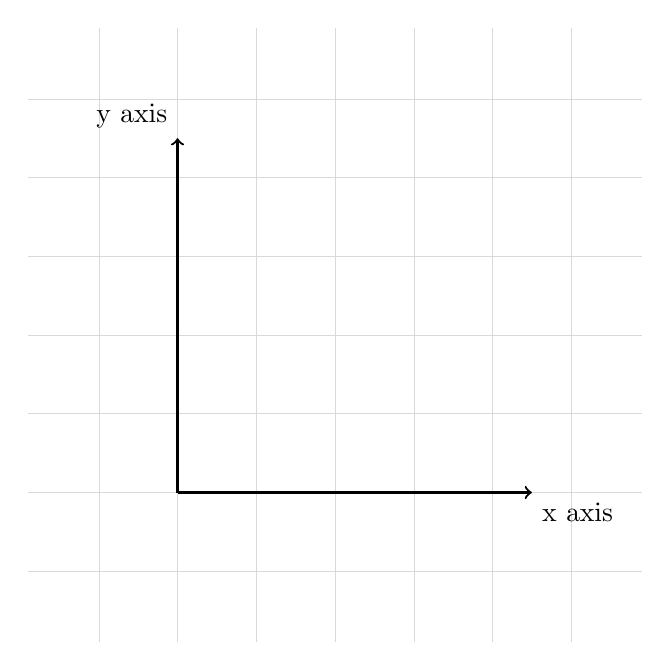
\begin{tikzpicture}
    \draw[step=1cm,gray!30,very thin] (-1.9,-1.9) grid (5.9,5.9);
   \draw[thick, ->] (0,0) -- (4.5,0) node[below right] {x axis};
   \draw[thick, ->] (0,0) -- (0,4.5) node[above left] {y axis};
\end{tikzpicture}
\end{center}

\end{minipage}%
}  
\end{center}

\vspace{20pt}


\begin{Verbatim}[fontsize=\footnotesize]
 \draw[thick, ->] (0,0) -- (4.5,0) node[below right] {x axis};
 \draw[thick, ->] (0,0) -- (0,4.5) node[above left]  {y axis};
\end{Verbatim}

\end{frame}

%%% KOORDINATSYSTEM: LABEL OG TALL%%%
\begin{frame}[fragile]
\frametitle{Rutenett med akser}
\begin{center}
\scalebox{0.5}{%
\begin{minipage}{\textwidth}
\begin{center}
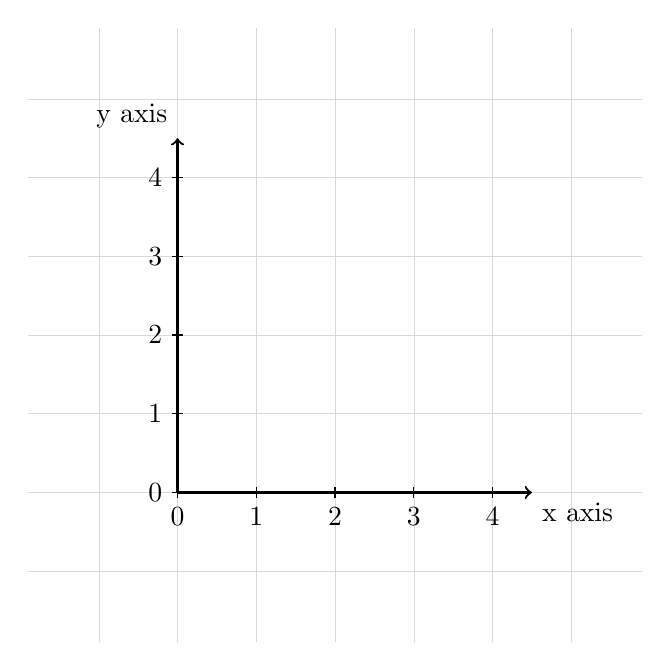
\begin{tikzpicture}
    \draw[step=1cm,gray!30,very thin] (-1.9,-1.9) grid (5.9,5.9);
    \draw[thick, ->] (0,0) -- (4.5,0) node[anchor=north west] {x axis};
    \draw[thick, ->] (0,0) -- (0,4.5) node[anchor=south east] {y axis};

    \foreach \x in {0,1,2,3,4}
	\draw (\x cm, 2pt) -- (\x cm, -2pt) node[anchor=north] {$\x$};
    \foreach \y in {0,1,2,3,4}
	\draw (2pt, \y cm) -- (-2pt, \y cm) node[anchor=east] {$\y$};
\end{tikzpicture}
\end{center}

\end{minipage}%
}  
\end{center}

\vspace{20pt}

\begin{Verbatim}[fontsize=\footnotesize]
\foreach \x in {0,1,2,3,4}
  \draw (\x cm, 2pt) -- (\x cm, -2pt) node[below] {$\x$};
\foreach \y in {0,1,2,3,4}
  \draw (2pt, \y cm) -- (-2pt, \y cm) node[left]  {$\y$};
\end{Verbatim}

\end{frame}

%%% TRÆR: ILLUSTRASJON %%%
\begin{frame}[fragile]
\frametitle{Trær}

\begin{center}
\begin{tikzpicture}[every node/.style={},
				   level 2/.style={sibling distance=20mm},
				   level 3/.style={sibling distance=10mm}, 
				   level distance=30pt]
\node {S}
	child { node{A} 
		child { node {A} 
			child { node {(} }
			child { node {)} }
		}
		child { node {A} 
			child { node {(} }
			child { node {A} 
				child { node {(} }
				child { node {)} }
			}
			child { node {)} }
		}
	};
\end{tikzpicture}
\end{center}

\end{frame}

%%% NODER: FASONGER %%%
\begin{frame}[fragile]
\frametitle{Noder -- fasonger}
\framesubtitle{\textbackslash usetikzpackage\{shapes\}}

\begin{center}
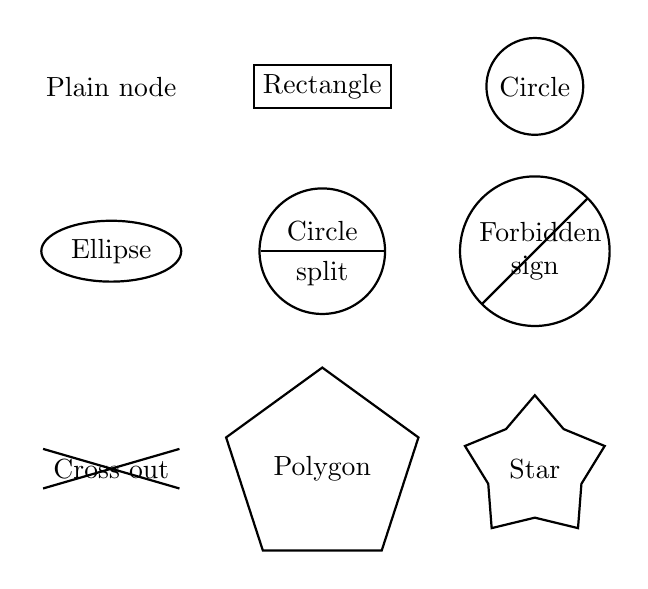
\begin{tikzpicture}
    \matrix[nodes={draw, thick},
        row sep=0.5cm,column sep=0.5cm] {
    \node[draw=none,fill=none] {Plain node}; &
    \node[rectangle] {Rectangle}; &
    \node[circle] {Circle};\\
    \node[ellipse] {Ellipse};&
    \node[circle split] {Circle \nodepart{lower} split};&
    \node[forbidden sign,text width=4em, text centered] {Forbidden sign};\\
    \node[cross out] {Cross out};&
    \node[regular polygon,regular polygon sides=5] {Polygon};&
    \node[star] {Star};\\
    };
\end{tikzpicture}
\end{center}

\end{frame}


%%% TRÆR: BYGGING %%%
\begin{frame}[fragile]
\frametitle{Trær -- bygge et tre}

Rot-noden:
\begin{center}
\begin{tikzpicture}[every node/.style={},level 2/.style={sibling distance=20mm},
				   level 3/.style={sibling distance=10mm}, level distance=30pt]
\node {1};
\end{tikzpicture}
\end{center}

\begin{Verbatim}[fontsize=\small]
\node {1};
\end{Verbatim}

Bygger videre:

\begin{center}
\begin{tikzpicture}[every node/.style={},level 1/.style={sibling distance=10mm},
				   level 3/.style={sibling distance=10mm}, level distance=25pt]
\node {1}
	child {node {2}}
	child {node {3}
		child {node {4} }
		child {node {5} }
	}
;
\end{tikzpicture}
\end{center}

\begin{Verbatim}[fontsize=\small]
\node {1}
    child { node {2} }
    child { node {3} 
        child { node {4} }
        child { node {5} }
    }
;
\end{Verbatim}


\end{frame}

%%% TRÆR: KODEN %%%
\begin{frame}[fragile]
\frametitle{Trær}

\begin{Verbatim}[fontsize=\footnotesize, frame=single]
\begin{tikzpicture}[every node/.style={},
                    level 2/.style={sibling distance=20mm},
                    level 3/.style={sibling distance=10mm}, 
                    level distance=30pt]
\node {S}
    child { node{A} 
        child { node {A} 
            child { node {(} }
            child { node {)} }
        }
        child { node {A} 
            child { node {(} }
            child { node {A} 
                child { node {(} }
                child { node {)} }
            }
            child { node {)} }
        }
    }
;
\end{tikzpicture}
\end{Verbatim}

\end{frame}

%%% TRÆR: RØD-SVART %%%
\begin{frame}[fragile]
\frametitle{Rød-svarte trær}


\tikzset{
	treenode/.style = {align=center, inner sep=0pt},
	% Sorte noder
  	node_black/.style = {treenode, circle, white, font=\bfseries, draw=black,fill=black, text width=0.8cm},
	% Røde noder
  	node_red/.style = {treenode, circle, red, draw=red, text width=0.8cm, very thick},
	% Null-pekere
  	node_null/.style = {treenode, rectangle, draw=black, minimum width=0.3cm, minimum height=0.3cm}
}

\begin{center}
% Skal tegne med piler (->), og setter level/.style={opt.} %
\begin{tikzpicture}[->,level/.style={sibling distance = 2cm, level distance = 1.5cm}] 
\node [node_black] {38}
    	child{ node [node_red] {19} 
		child{node [node_black] {12}
			child{node [node_red] {8}}
			child{node [node_null] {}}
		}
		child{node [node_black] {31}}
	}
    	child{ node [node_black] {41} }
; 
\end{tikzpicture}
\end{center}

\end{frame}

%%% TRÆR: RØD-SVART STIL KODE %%%
\begin{frame}[fragile]
\frametitle{Trær}

\begin{Verbatim}[fontsize=\footnotesize, frame=single]
\tikzset{
   treenode/.style = {align=center, inner sep=0pt},
	
   % Sorte noder
   node_black/.style = {treenode, circle, white, 
		                  	     font=\bfseries, draw=black,
			                        fill=black, text width=0.8cm},
   % Røde noder
   node_red/.style = {treenode, circle, red, draw=red, 
	                      text width=0.8cm, very thick},
   % Null-pekere
   node_null/.style = {treenode, rectangle, draw=black, 
		                       minimum width=0.3cm, 
                       minimum height=0.3cm}
}
\end{Verbatim}

\end{frame}


%%% TRÆR: RØD-SVART KODE %%%
\begin{frame}[fragile]
\frametitle{Trær}

\begin{Verbatim}[fontsize=\footnotesize, frame=single]
\begin{tikzpicture}[->,level/.style={ sibling distance = 2cm, 
                    level distance = 1.5cm }] 

\node [node_black] {38}
    child {node [node_red] {19} 
        child {node [node_black] {12}
             child {node [node_red] {8} }
             child {node [node_null] {} }
        }
        child {node [node_black] {31} }
    }
    child { node [node_black] {41} }
; 
\end{tikzpicture}
\end{Verbatim}

\end{frame}


%%% GRAFER %%%
\begin{frame}[fragile]
\frametitle{Grafer}

\begin{center}
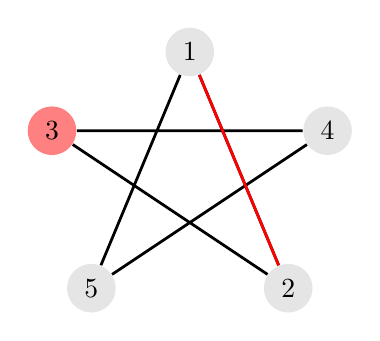
\begin{tikzpicture}[scale=5]
	 \tikzstyle{vertex}=[circle,fill=black!10]
	 \tikzstyle{selected vertex} = [vertex, fill=red!50]

	 \tikzstyle{selected edge} = [draw,line width=1pt,-,red!100]
	 \tikzstyle{edge} = [-,black,line width=1pt]

	 \node[vertex] (v1) at (1.25,1.7) 			{1};
	 \node[vertex] (v2) at (1.5,1.1) 				{2};
	 \node[selected vertex] (v3) at (0.9,1.5) 		{3};
	 \node[vertex] (v4) at (1.6,1.5) 				{4};
	 \node[vertex] (v5) at (1,1.1) 				{5};

	\draw[edge] (v1)  -- (v2) -- (v3) -- (v4) -- (v5) -- (v1); 
	\draw[selected edge] (v1) -- (v2);
\end{tikzpicture}
\end{center}

\begin{itemize}
\item
Noder (\texttt{vertex}) 
\item
Markerte noder (\texttt{selected vertex})
\item
Kanter (\texttt{edge})
\item
Markerte kanter (\texttt{selected edge})
\end{itemize}

\end{frame}


%%% GRAFER : NODER %%%
\begin{frame}[fragile]
\frametitle{Grafer -- noder}

\begin{center}

\begin{tikzpicture}[scale=5]
	 \tikzstyle{vertex}=[circle,fill=black!10]
	 \tikzstyle{selected vertex} = [vertex, fill=red!50]

	 \tikzstyle{selected edge} = [draw,line width=1pt,-,red!100]
	 \tikzstyle{edge} = [-,black,line width=1pt]

	 \node[vertex] (v1) at (0,0) {1};
	\node[selected vertex] (v2) at (0.5,0) {2};
\end{tikzpicture}
\end{center}

\begin{Verbatim}[fontsize=\small]
\tikzstyle{vertex} = [circle,fill=black!10]
\tikzstyle{selected vertex} = [vertex, fill=red!50]

% Tegne nodene
\node[vertex]          (v1) at (0,0)   {1};
\node[selected vertex] (v2) at (0.5,0) {2};
\end{Verbatim}

\end{frame}

%%% GRAFER : KANTER %%%
\begin{frame}[fragile]
\frametitle{Grafer -- kanter}

\begin{center}
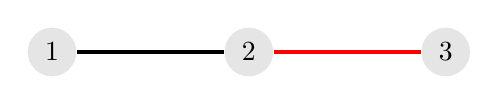
\begin{tikzpicture}[scale=5]
	 \tikzstyle{vertex}=[circle,fill=black!10]
	 \tikzstyle{selected vertex} = [vertex, fill=red!50]

	 \tikzstyle{selected edge} = [draw,line width=1.5pt,-,red!100]
	 \tikzstyle{edge} = [-,black,line width=1.5pt]

	 \node[vertex] (v1) at (0,0) {1};
	\node[vertex] (v2) at (0.5,0) {2};
	\node[vertex] (v3) at (1,0) {3};

	\draw[edge] (v1) -- (v2);
	\draw[selected edge] (v2) -- (v3);
\end{tikzpicture}
\end{center}

\begin{Verbatim}[fontsize=\small]
\tikzstyle{selected edge} = [draw,line width=1pt,-,red!100]
\tikzstyle{edge} = [-,black,line width=1pt]

% Tegne nodene
\node[vertex] (v1) at (0,0)   {1};
\node[vertex] (v2) at (0.5,0) {2};
\node[vertex] (v3) at (1,0)   {3};

% Tegne kantene
\draw[edge]          (v1) -- (v2);
\draw[selected edge] (v2) -- (v3);
\end{Verbatim}

\end{frame}

%%% GRAFER : KANTER %%%
\begin{frame}[fragile]
\frametitle{Grafer -- kanter}


\begin{Verbatim}[fontsize=\footnotesize, frame=single]
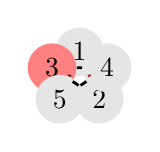
\begin{tikzpicture}
    \tikzstyle{vertex}         = [circle,fill=black!10]
    \tikzstyle{selected vertex}= [vertex, fill=red!50]

    \tikzstyle{selected edge}  = [draw,line width=1pt,-,red!100]
    \tikzstyle{edge}           = [-,black,line width=1pt]

    \node[vertex]          (v1) at (1.25,1.7) {1};
    \node[vertex]          (v2) at (1.5,1.1)  {2};
    \node[selected vertex] (v3) at (0.9,1.5)  {3};
    \node[vertex]          (v4) at (1.6,1.5)  {4};
    \node[vertex]          (v5) at (1,1.1)    {5};

    \draw[edge]          (v1)--(v2)--(v3)--(v4)--(v5)--(v1); 
    \draw[selected edge] (v1)--(v2);
\end{tikzpicture}
\end{Verbatim}

\end{frame}


%%% AUTOMATER %%%
\begin{frame}[fragile]
\frametitle{Automater}


\begin{center}
\scalebox{0.8}{%
\begin{minipage}{\textwidth}
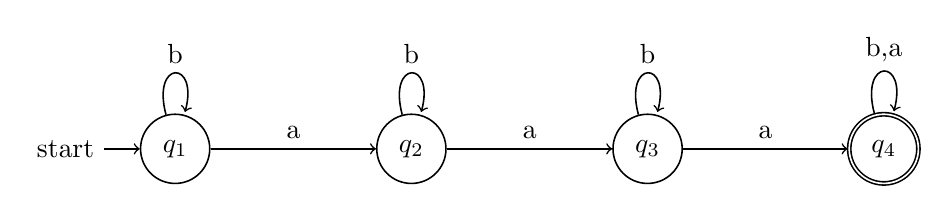
\begin{tikzpicture}[->,auto,node distance=3cm,line width=0.2mm]
  \node[initial,state] 			(A)		 	         {$q_1$};
  \node[state]         			(B) [right of=A] 	{$q_2$};
  \node[state]				(C) [right of=B] 	{$q_3$};
  \node[state,accepting]		(D) [right of=C] 	{$q_4$};

  \path 	(A) edge [loop above] node 			{b} 		(A)
			edge node 						{a} 		(B)
        		(B) edge [loop above] node 			{b} 		(B)
			edge node 						{a} 		(C)
		(C) edge [loop above] node 			{b}		(C)
			edge node 						{a} 		(D)
		(D) edge [loop above] node 			{b,a}	(D);
\end{tikzpicture}
\end{minipage}%
}  
\end{center}

Må inkludere \texttt{\textbackslash usetikzlibrary\{automata\}}.

\end{frame}

%%% AUTOMATER: KODE %%%
\begin{frame}[fragile]
\frametitle{Automater}


\begin{Verbatim}[fontsize=\footnotesize, frame=single]
\begin{tikzpicture}[->,auto,node distance=3cm,line width=0.2mm]
  \node[initial,state   (A) 	          	    {$q_1$};
  \node[state]          (B) [right of=A]    {$q_2$};
  \node[state]	         (C) [right of=B]    {$q_3$};
  \node[state,accepting](D) [right of=C]    {$q_4$};

  \path (A) edge [loop above] node 	 {b}   (A)
	    edge node      			                 {a}   (B)
        (B) edge [loop above] node 	 {b}   (B)
	    edge node   	                    {a}   (C)
        (C) edge [loop above] node	  {b}   (C)
	    edge node 	    	                 {a}   (D)
        (D) edge [loop above] node 	 {b,a} (D);
\end{tikzpicture}
\end{Verbatim}

\end{frame}


%%% ANDRE TIKZ-BIBLIOTEKER %%%
\begin{frame}[fragile]
\begin{center}
\Huge{Andre TikZ-biblioteker}
\end{center}
\end{frame}

% mindmap
\begin{frame}[fragile]
\frametitle{\texttt{mindmap}}

\begin{center}
\scalebox{0.6}{
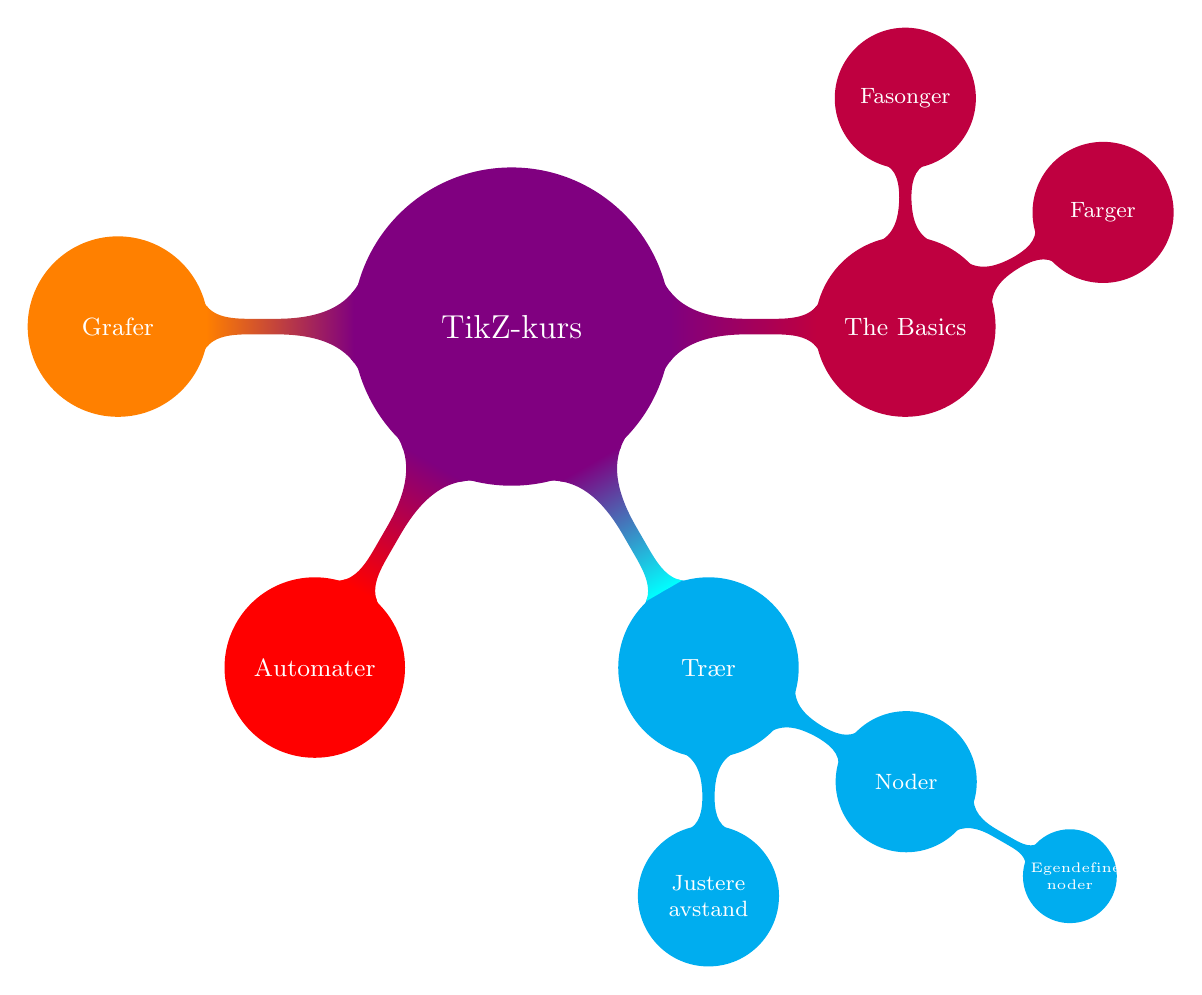
\begin{tikzpicture}
  \path[mindmap,concept color=violet,text=white]
    node[concept] {TikZ-kurs}
    [clockwise from=0]
    child[concept color=purple] {
      node[concept] {The Basics}
      [clockwise from=90]
      child { node[concept] {Fasonger} }
      child { node[concept] {Farger} }
    }  
    child[concept color=cyan] {
      node[concept] {Trær}
      [clockwise from=-30]
      child { node[concept] {Noder} 
		child { node[concept] {Egendefinerte noder}}
	}
      child { node[concept] {Justere avstand} }
    }
    child[concept color=red] { node[concept] {Automater} }
    child[concept color=orange] { node[concept] {Grafer} };
\end{tikzpicture}
}
\end{center}

\end{frame}

\begin{frame}[fragile]
\frametitle{\texttt{mindmap}}

\begin{Verbatim}[fontsize=\scriptsize, frame=single]
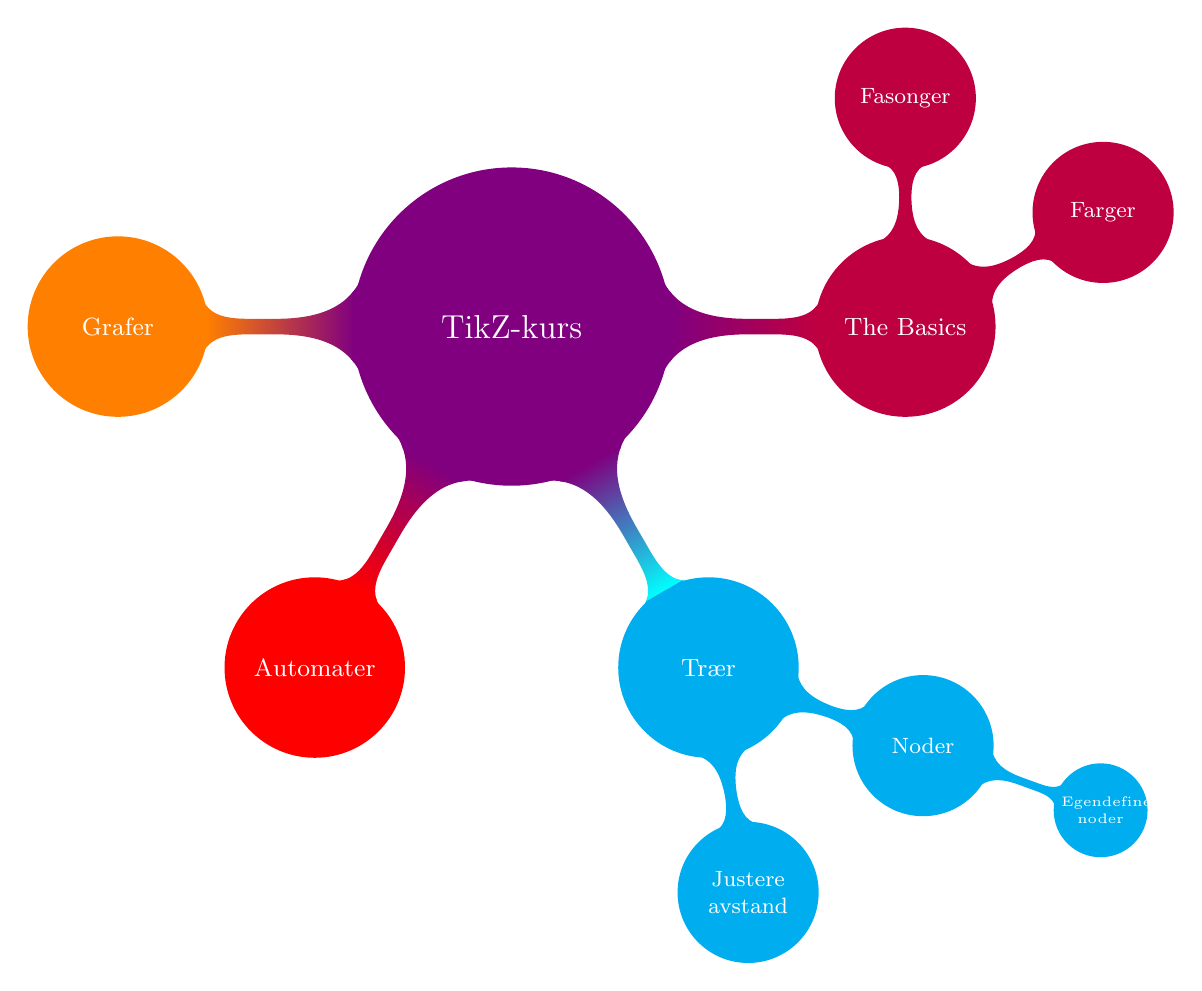
\begin{tikzpicture}
\path[mindmap,concept color=violet,text=white]
    node[concept] {TikZ-kurs}
    [clockwise from=0]
    child[concept color=purple] { 
    node[concept] {The Basics} [clockwise from=90]
        child { node[concept] {Fasonger} }
        child { node[concept] {Farger} }
    }  
    child[concept color=cyan] {
    node[concept] {Trær} [clockwise from=-20]
        child { node[concept] {Noder} 
            child { node[concept] {Egendefinerte noder}}
        }
        child { node[concept] {Justere avstand} }
     }
    child[concept color=red] { node[concept] {Automater} }
    child[concept color=orange] { node[concept] {Grafer} };
\end{tikzpicture}
\end{Verbatim}

\end{frame}

% calendar
\begin{frame}[fragile]
\frametitle{\texttt{calendar}}

\begin{center}

\begin{tikzpicture}[every day/.style={anchor=mid}]
\calendar (mycalendar) [dates=2016-11-01 to 2016-11-30,week list, 
					    month label above centered,
					    month text=\textcolor{teal}{\%mt} \%y-] 
					    if (Sunday) [red]
					    if (equals=2016-11-01) {\draw[red,thick] (0,0) circle (7pt);};
\end{tikzpicture}
\end{center}

\begin{Verbatim}[fontsize=\scriptsize, frame=single]

\begin{tikzpicture}
\calendar (mycalendar) [dates=2016-11-01 to 2016-11-30,week list, 
					    month label above centered,
					    month text=\textcolor{teal}{\%mt} \%y-] 
					    if (Sunday) [red]
					    if (equals=2016-11-01) {\draw[red,thick] (0,0) circle (7pt);};
\end{tikzpicture}
\end{Verbatim}

\end{frame}


\begin{frame}
Takk for meg!

\vspace{20pt}

\textbf{Lære mer?}
\begin{itemize}
\item
TeXample.net
\item
tug.org
\end{itemize}
\end{frame}


\end{document}